\documentclass[12pt,a4paper]{article}
\usepackage[utf8]{inputenc}
\usepackage{amsmath}
\usepackage[brazilian]{babel} % Brazil or not Brazil??
\usepackage{amsfonts}
\usepackage{amssymb}
\usepackage{graphicx}
\usepackage[margin=0.8in]{geometry}


\begin{document}
\title{\vspace{70mm}\Huge Experimento 05 - Viscosidade - Lei de Stokes}
\author{ Giovani Garuffi\qquad\hfill
		\textit {RA: 155559}\protect\\
		João Baraldi\hfill
		\textit{RA: 158044}\protect\\
		Lauro Cruz\hfill
		\textit{RA: 156175}\protect\\
		Lucas Schanner\hfill
		\textit{RA: 156412}\protect\\
		Pedro Stringhini\hfill
		\textit {RA: 156983}								
		}
\maketitle
\newpage
\section{Resumo}
O experimento consistiu em soltar pequenas esferas de aço com diâmetros variados (previamente medidos em um micrômetro) na parte superior de um cilindro preenchido com uma solução de água e glicerina, para que assim que elas atingissem uma velocidade estável, essa fosse calculada a partir da medição do tempo necessário para percorrer um trecho específico marcado.
Após as devidas repetições do procedimento para as várias esferas, foi possível calcular a velocidade estável de cada esfera e por meio da fórmula:
$$v_L = (\frac{2}{9}) (\frac{\rho - \rho'}{\eta}) g r^2$$
Sendo que, para minimizar os erros, a velocidade deveria ser multiplicada por
$$K = (1 + \frac{2.4r}{A})(1 + \frac{3.3r}{H})$$
Foi possível a obtenção do coeficinte de viscosidade da solução, assim como a porcentagem de glicerina presente no cilindro.

\section{Objetivos}
Esse experimento tem como objetivo calcular o coeficiente de viscosidade de uma solução de glicerina em água, e sua porcentagem em massa.


\section{Procedimento Experimental e Coleta de Dados}


\subsection{Procedimento}

O experimento é composto basicamente por um cilíndro de vidro preenchido com uma solução de glicerina, até uma altura $H$, que está preso em suporte graduado com maracs ajustáveis que distam entre si $L$ (no caso, $H = (42.50 \pm 0.05) \; cm$ e $L = (20 \pm 0.05) \; cm$). Dentro do tubo há, também, um termômetro de mercúrio para controle e conhecimento da temperatura da solução. Há, ainda, um conjunto de cinco esferas de aço de diâmetros previamente mensurados com um micrômetro (para então obter-se o raio $r$). Vide figura \ref{experimento}.\\

Então, com auxílio de uma pinça, uma esfera é abandonada na superfície do líquido, e quando ela atinge a altura da primeira marca ajustável, distante da superficie o suficiente para a normalização da velocidade de queda da esfera (velocidade limite $v_L$), inicia-se o cronômetro e mede-se o tempo que a esfera leva até a segunda marca. Esse procedimento foi ralizado cinco vezes para cada esfera.\\

\begin{figure}[!htbp]
\centering
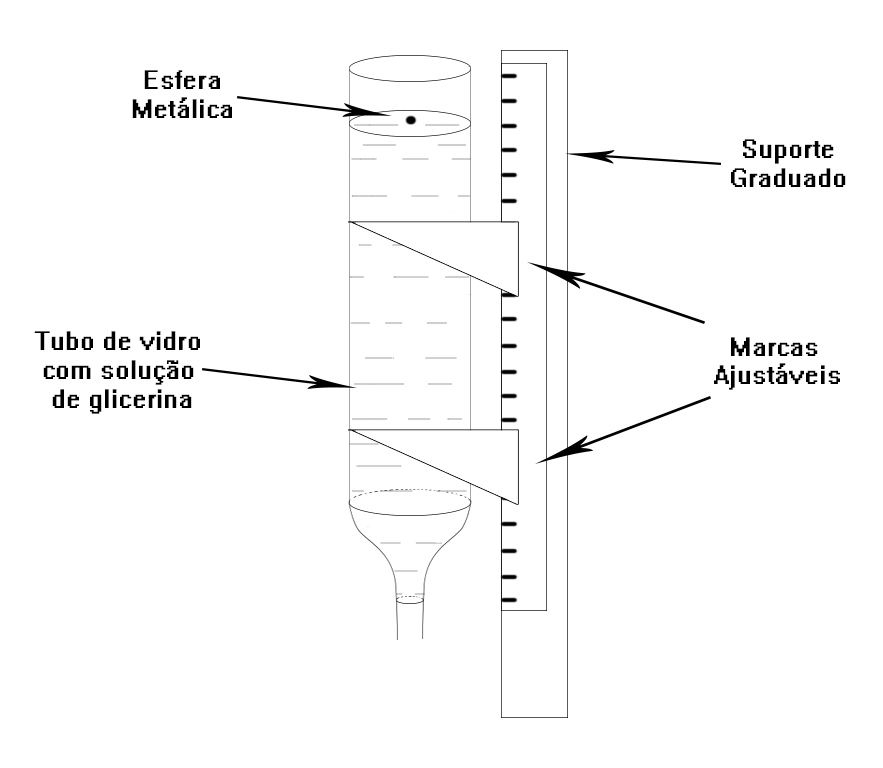
\includegraphics[scale=0.3]{Fig5-1.jpg}
\caption{Exemplo da montagem experimental.}
\label{experimento}
\end{figure}

Então, através da relação

$$v_L = (\frac{2}{9}) (\frac{\rho - \rho'}{\eta}) g r^2$$

onde $ \rho = 782 \pm 1  \dfrac{Kg}{m^3} $ é a densidade da esfera, $ \rho' = 120 \pm 10 \dfrac{Kg}{m^3} $ a do meio (ambas previamente conhecidas, $\eta$ é o coeficiente de viscosidade do meio, e $g$ é a aceleração da gravidade local, podemos descobrir o valor de $\eta$.\\

Entretanto, o cilindro de vidro interfere no movimento da esfera, de modo que a velocidade da esfera no tubo é reduzida de acordo com o fator de Ladenburg

$$K = (1 + \frac{2.4r}{A})(1 + \frac{3.3r}{H})$$

onde $A$ é o raio do cilindro, obtido pelo diâmetro, medido com um paquímetro.

Então, para a velocidade medida, $v_L'$, convir com a primeira equação, temos que multiplicá-la por $K$, deste modo

$$v_L = Kv_L = (\frac{2}{9}) (\frac{\rho - \rho'}{\eta}) g r^2$$

Então, com o valor de $\eta$ e a temperatura, pode-se obter a porcentagem, em massa, de glicerina na solução, pela análise do gráfico da figura \ref{porcentagem}, retirado da bibliografia 1, presente na apostila do experimento.\\

\begin{figure}[!htbp]
\centering
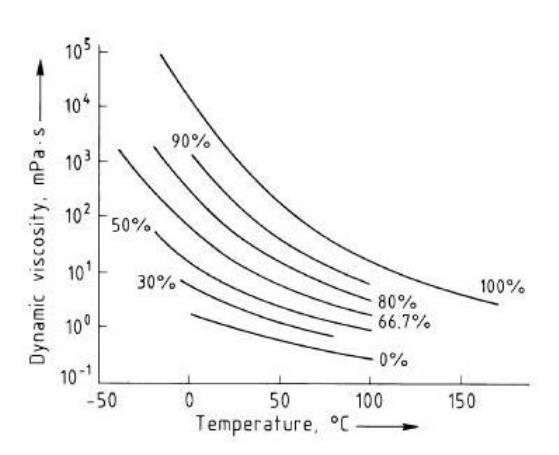
\includegraphics[scale=0.4]{Fig5-2.jpg}
\caption{Viscosidade da mistura glicerina-água. As concentrações
são dadas em percentual de massa de glicerina.}
\label{porcentagem}
\end{figure}

\subsection{Dados Obtidos}

A Tabela \ref{dados} apresenta as medições do tempo de queda de cada esfera, relacionada ao seu raio.

\begin{table}[!htbp]

\centering
\def\arraystretch{1.5}
\caption{Dados obtidos no experimento}

\begin{tabular}{|c|rrrrr|r|}
\hline
$ r \; (m)$ & \multicolumn{5}{c|}{Medidas de $T$ \;  (s)} & $T_{medio} \; (s)$  \\
\hline
  $ 0.00100 \pm 0.00005 $ &12.47 & 12.22 & 11.87 & 11.97 & 11.94 & $ 12.0 \pm 0.3 $ \\
  \hline
  $ 0.00125 \pm 0.00005 $ &7.65 & 7.87 & 7.59 & 7.60 & 7.78  & $ 7.7 \pm 0.3 $   \\
  \hline
  $ 0.00150 \pm 0.00005 $ &5.46 & 5.29 & 5.35 & 5.69 & 5.32 & $ 5.4 \pm 0.3 $     \\
  \hline
  $ 0.00175 \pm 0.00005 $ &4.07 & 4.15 & 4.09 & 4.09 & 4.13  & $ 4.1 \pm 0.3 $    \\
  \hline
  $ 0.00200 \pm 0.00005 $ &3.12 & 3.25 & 3.28 & 3.28 & 3.25 & $ 3.2 \pm 0.3 $       \\
\hline
\end{tabular}

\emph{O erro instrumental em $T$ é considerado $0.3$ devido às dificuldades em realizar as medições}
\label{dados}
\end{table}




\section{Análise dos Resultados e Discussões}
\subsection{Regressão linear}
O situação estudada pode ser modelada a partir da equação: 

$$ v_l = \frac{2}{9} \frac{(\rho - \rho ')}{\eta}g \cdot r^2$$

Obtida a partir da força de empuxo, força gravitacional e da Lei de Stokes. $\rho$ e $\rho '$ são as densidades da esfera e do meio, respectivamente e $\eta$ é o coeficiente de viscosidade do meio.

No entanto a velocidade precisa ser corrigida pelo fator de Landenburg
$$ v_l = K \cdot v_l ' = K \frac{L}{t}$$
$$ \Delta v_l = \sqrt{\frac{K^{2} L^{2}}{t^{4}} \Delta{t}^{2} + \frac{K^{2} \Delta{L}^{2}}{t^{2}} + \frac{L^{2} \Delta{K}^{2}}{t^{2}}} $$
Onde K é o fator de Landenburg, dado por 
$$ K = \left(1 + \frac{3.3 r}{H}\right) \left(1 + \frac{2.4 r}{ \pi r_{c}^{2}}  \right) $$
$$ \Delta K = $$
$$\sqrt{\frac{23.04 \Delta{r_{c}}^{2} r^{2}}{\pi^{2} r_{c}^{6}} \left(1 + \frac{3.3 r}{H}\right)^{2} + \Delta{r}^{2} \left(\frac{2.4 + \frac{7.92 r}{H}}{\pi r_{c}^{2}} + \frac{1}{H} \left(\frac{7.92 r}{\pi r_{c}^{2}} + 3.3\right)\right)^{2} + \frac{10.89 \Delta{H}^{2}}{H^{4}} r^{2} \left(\frac{2.4 r}{\pi r_{c}^{2}} + 1\right)^{2}} $$




Na equação  vemos que existe uma relação linear entre $v_l$ e $r^2$. Para explorar essa relação, foi construída a Tabela \ref{linear}, relacionando $v_l$ a $ r^2 $ .

\begin{table}[!htbp]
\centering
\def\arraystretch{1.5}
\caption{Raio ao quadrado relacionado à velocidade máxima de uma esfera em liquido viscoso}
\begin{tabular}{|c|c|c|c|c|}
\hline
$r \; (m)$ & $r^2 \; (m^2)$ & $T_{queda} \; (s)$ & $ K $ & $ v_l \; (m/s)$  \\

\hline
$ 0.00100 \pm 0.00005 $ & $1.0 \cdot 10^{-6} \pm 1 \cdot 10^{-7}$   &$ 12.0 \pm 0.3$ & $ 1.85 \pm 0.04$ & $0.030 \pm 0.001 $\\
 \hline
$ 0.00125 \pm 0.00005 $ & $1.5 \cdot 10^{-6} \pm 1 \cdot 10^{-7}$ & $ 7.7 \pm 0.3$ & $ 2.07 \pm 0.04$  & $0.053 \pm 0.002 $\\
 \hline
$ 0.00150 \pm 0.00005 $ & $2.2 \cdot 10^{-6} \pm 2 \cdot 10^{-7}$ & $ 5.4 \pm 0.3$ & $ 2.28 \pm 0.04$  & $0.084 \pm 0.005 $\\
 \hline
$ 0.00175 \pm 0.00005 $ & $3.0 \cdot 10^{-6} \pm 2 \cdot 10^{-7}$ & $ 4.1 \pm 0.3$ & $ 2.50 \pm 0.04$   & $0.121 \pm 0.009 $ \\
 \hline
 $0.00200 \pm 0.00005 $ & $4.0 \cdot 10^{-6} \pm 2 \cdot 10^{-7}$   & $ 3.2 \pm 0.3$ & $ 2.71 \pm 0.04$   & $0.16 \pm 0.01 $\\
\hline
\end{tabular}

\emph{O erro em T foi calculado pelo erro estatístico e utilizando como  erro instrumental $\pm 0.3$.}
 
\label{linear}
\end{table}

Fazendo a regressão linear de $ v_l$ X $ r^2 $, pelo método de mínimos quadrados, obtém-se os seguintes coeficientes: 
	$$ a = (41 \pm 2) \cdot 10^3  \;\; (1/ms)$$
	$$ b = 0.011 \pm 0.003 \; (m/s).$$

A reta resultante da regressão linear, sobreposta aos pontos medidos experimentalmente pode ser vista na Figura \ref{grafico}.

\begin{figure}
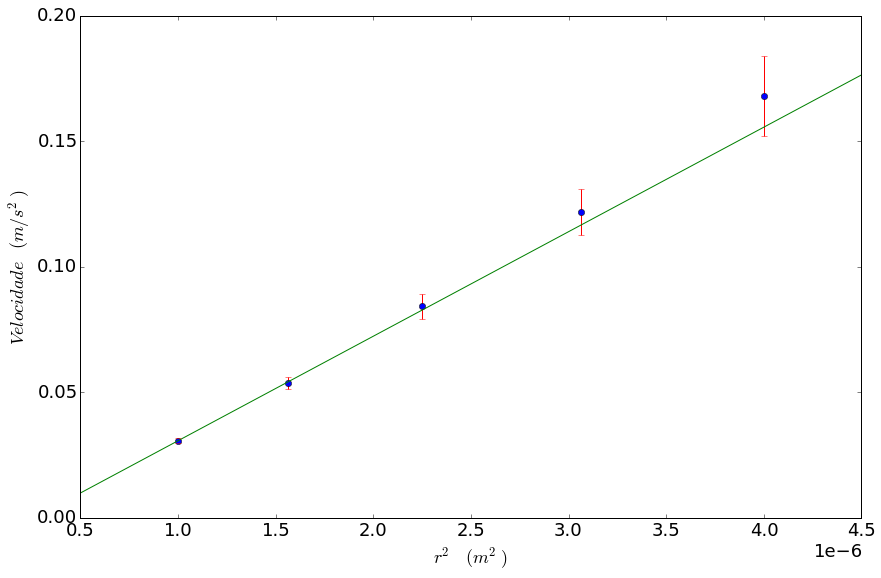
\includegraphics[scale=0.55]{grafico.png}
\caption{Regressão linear de $v_t$ por $r^2$ sobreposta aos pontos experimentais}
\label{grafico}
\end{figure}

\subsection{Significado físico do coeficiente angular}
O coeficiente angular  é equivalente a
$$a = \frac{2}{9} \frac{(\rho - \rho ')}{\eta}g,$$ 
o que implica que 
$$\eta = \frac{2}{9} \frac{(\rho - \rho ')}{a}g,$$
$$\Delta\eta = \frac{2}{9}\sqrt{g^2\frac{(\rho - \rho ')^2}{a^4} \cdot \Delta a^2 + \frac{(\rho - \rho ')^2}{a^2}\cdot \Delta g^2 + \frac{g^2}{a^2} \cdot \Delta \rho ^2 + \frac{g^2}{a^2} \cdot \Delta \rho '^2}. $$
Considerando $ g = 9.8 \pm 0.1 $:
$$\eta = 0.35 \pm 0.02 \dfrac{Kg}{m \cdot s} $$


\section{Conclusões}


\section{Bibliografia}
1.\textit{Ullmann's Encyclopedia of Industrial Chemistry}, Vol. A12, p. 479. (Biblioteca do
IQ, Unicamp $\#$ R660 ULM5 IQ/10.183 V.A12).

\end{document}

